\section{Appendix}

\subsection*{Appendix A: Variational Inference}

In line with \cite{wang2013variational}, consider a generic topic model with latent variables $\theta$ and $z$ as well as observed data $x$:
\begin{align*}
p(\theta,z,x) &= p(x|z)p(z|\theta)p(\theta).
\end{align*}
The exact posterior distribution
\begin{align*}
p(\theta,z|x) &= \frac{p(\theta,z,x)}{\int p(\theta,z,x)dzd\theta}
\end{align*}
is usually intractable due to the high-dimensional integral, which is why the distribution needs to be approximated.

As stated in section 2.3, in variational inference a simple distribution family $q(\theta,z)$ is posited and subsequently, we determine the member of this family - that is, the variational parameter(s) - that minimizes the KL divergence. Note that, for computational purposes, we compute KL divergence of the true posterior $p$ from the approximating posterior $q$, $\text{KL}(q||p)$, whereas intuitively one would seek to minimize $\text{KL}(p||q)$.

The most popular variational inference technique is mean-field variational inference (also: mean-field variational Bayes), where we posit full factorizability of $q(\theta,z)$: $q(\theta,z) = q(\theta)q(z)$. That is, $\theta$ and $z$ are assumed to be independent with their own distributions and variational parameters $\phi$ (which we suppress for improved readability). Since $\theta$ and $z$ are actually dependent, this approximate distribution family $q(\theta,z)$ does not contain the true posterior $p(\theta,z|x)$.  

Let us now write out the KL divergence of $p$ from $q$:
\begin{align*}
\text{KL}(q||p) &= \mathbb{E}_q[\log\frac{q(\theta,z)}{p(\theta,z|x)}] \\
&= \mathbb{E}_q[\log q(\theta,z)] - \mathbb{E}_q[\log p(\theta,z|x)] \\
&=\mathbb{E}_q[\log q(\theta,z)] - \mathbb{E}_q[\log p(\theta,z,x)] + \log p(x) 
\end{align*}
Since $\text{KL}(q||p) \geq 0$ (which can be easily shown using Jensen's inequality), it follows that:
\begin{align*}
\log p(x) & \geq \mathbb{E}_q[\log p(\theta,z,x)] - \mathbb{E}_q[\log q(\theta,z)].
\end{align*}
The left-hand side of the above inequality is the marginal log likelihood of observed data $x$ and is also called evidence (of the observed data). Note that the evidence is not computable - otherwise we would not need to resort to variational inference in the first place. The right-hand side thus presents a lower bound on the evidence and we define the \textit{Evidence Lower BOund} (ELBO) as:
\begin{align*}
\text{ELBO} := \mathbb{E}_q[\log p(\theta,z,x)] - \mathbb{E}_q[\log q(\theta,z)],
\end{align*}
where the second component of the ELBO, $\mathbb{E}_q[\log q(\theta,z)$, is the entropy of the approximate distribution $q$. Equivalently, we could say that the evidence constitutes an upper bound for the ELBO. This means that we actively maximize the ELBO (which is therefore also called \textit{variational objective}), which in turn is equivalent to minimizing the KL divergence of the true posterior $p(\theta,z|x)$ from the approximate distribution $q(\theta,z)$. Therefore, the approximation $q(\theta,z)$ - or, more precisely, the variational parameters $\phi$ of $q(\theta)$ and $q(z)$ - that maximizes the ELBO simultaneously minimizes KL divergence (\citealp{blei2003latent, wang2013variational}). \cite{wang2013variational} show that for the chosen factorization of the joint distribution $p(\theta,z,x)$, and using the optimality conditions as derived in \cite{bishop2006pattern}, we obtain the following solutions when setting $\frac{\partial \text{ELBO}}{\partial q}\overset{!}{=}0$:
\begin{align*}
q^{*}(\theta) \propto \exp\{\mathbb{E}_{q(z)}[\log p(z|\theta))p(\theta)]\}, \\
q^{*}(z) \propto \exp\{\mathbb{E}_{q(\theta)}[\log p(x|z))p(z|\theta)]\}.
\end{align*}
The coordinate ascent algorithm iteratively updates one of these two expressions while holding the other one constant, but requires closed-form updates to do so. This requirement is fulfilled as long as all model nodes are conditionally conjugate, i.e., as long as for each node in the model "its conditional distribution given its Markov blanket (i.e., the set of random variables that it is dependent on in the posterior) is in the same family as its conditional distribution given its parents (i.e., its factor in the joint distribution)" (\cite{wang2013variational}, p.\ 1008). The authors consequently define a class of models where some nodes are not conditionally conjugate, the so-called \textit{nonconjugate models}; for this class, using Laplace approximations, the variational family is shown to be $q(\theta,z) = q(\theta|\mu,\Sigma)q(z|\phi)$; that is, $q(\theta)$ is now Gaussian with variational parameters $\mu$ and $\Sigma$.

The STM in particular constitutes a nonconjugate model, since $p(\boldsymbol{\theta})$ is logistic normal and thus not conjugate with respect to the multinomial distribution $p(\boldsymbol{z}|\boldsymbol{\theta})$. Consequently, no closed-form update is available for $q(\boldsymbol{\eta})$. Using mean-field variational inference, the approximate posterior family is $\prod_{d=1}^{D}q(\boldsymbol{\eta}_d)q(\boldsymbol{z}_d)$, where $q(\boldsymbol{\eta}_d)$ is Gaussian and $q(\boldsymbol{z})$ is binomial (\citealp{roberts2016model}). Given the posterior, inference now consists in finding the particular member of the posterior distribution family that maximizes the approximate ELBO. (Due to the subsequent Laplace approximation, ELBO does not constitute a true lower bound on the evidence and the updates do not maximize ELBO directly, which is why \cite{roberts2013structural} use the term \textit{approximate} ELBO. See \cite{wang2013variational} for further discussion.) Applying Laplace variational inference, we approximate $q(\boldsymbol{\eta}_d)$ using a (quadratic) Taylor expression around the maximum-a-posteriori (MAP) estimate $\hat{\boldsymbol{\eta}}_d$, which yields a Gaussian variational posterior $q(\boldsymbol{\eta}_d)$, centered around $\hat{\boldsymbol{\eta}}_d$, and allows for a closed-form solution of $q(\boldsymbol{z}_d)$. Iteratively updating $q(\boldsymbol{\eta}_d)$ and $q(\boldsymbol{z}_d)$ thus constitutes the E-step of the EM algorithm.

The M-step consists in maximizing the approximate ELBO with respect to model parameters. Prevalence parameters $\boldsymbol{\Gamma}$ and $\boldsymbol{\Sigma}$ are updated through linear regression and maximum likelihood estimation (MLE), respectively. The updates for topic-word distributions $\boldsymbol{\beta}_k$ (or $\boldsymbol{\beta}_{k,a}$ if a content covariate is specified) are obtained through multinomial logistic regression. Further details are provided in \cite{roberts2013structural} and in the appendix of \cite{roberts2013structural}. Moreover, the appendix of \cite{blei2003latent} provides a detailed description of variatonal inference and empirical parameter estimation for the (conditionally conjugate) LDA model.

\subsection*{Appendix B: Additional Tables and Figures}

\subsubsection*{Additional Figures and Tables of Section 4}

\begin{center}
\begin{longtable}{|l|}
\captionsetup{justification=centering,margin=2cm}
\endlastfoot
\hline
\textit{Topic 1 Top Words:}\\
 	 \textbf{Highest Prob:} buerg, link, merkel, frau, sich \\
 	 \textbf{FREX:} altpartei, islam, linksextremist, asylbewerb, linksextrem \\
 	 \textbf{Lift:} eitan, 22jaehrig, abdelsamad, abgehalftert, afdforder \\
 	 \textbf{Score:} altpartei, linksextremist, frauenkongress, islamist, boehring \\
\hline
\textit{Topic 2 Top Words:}\\
 	 \textbf{Highest Prob:} frag, einfach, find, genau, halt \\
 	 \textbf{FREX:} geles, tweet, sorry, quatsch, lustig \\
 	 \textbf{Lift:} baseball, demjen, duitsland, garn, haeh \\
 	 \textbf{Score:} schmunzel, tweet, fuerstenberg, sorry, geles \\
\hline
\textit{Topic 3 Top Words:}\\
 	 \textbf{Highest Prob:} brauch, wichtig, leid, dank, klar \\
 	 \textbf{FREX:} emissionshandel, soli, marktwirtschaft, feedback, co2steu \\
 	 \textbf{Lift:} aequivalenz, altersvorsorgeprodukt, bildungsqualitaet, co2limit, co2meng \\
 	 \textbf{Score:} emissionshandel, co2limit, basisrent, euet, technologieoff \\
\hline
\textit{Topic 4 Top Words:}\\
 	 \textbf{Highest Prob:} sozial, miet, kind, arbeit, brauch \\
 	 \textbf{FREX:} mindestlohn, miet, wohnungsbau, mieterinn, loehn \\
 	 \textbf{Lift:} auseinanderfaellt, baugipfel, bestandsmiet, billigflieg, binnennachfrag \\
 	 \textbf{Score:} miet, mieterinn, mietendeckel, grundsicher, bezahlbar \\
\hline
\textit{Topic 5 Top Words:}\\
 	 \textbf{Highest Prob:} digital, jung, duesseldorf, bildung, christian \\
 	 \textbf{FREX:} fdpbundestagsabgeordnet, duesseldorf, rimkus, intelligenz, startups \\
 	 \textbf{Lift:} boeing, dettenheim, duesseldorfbilk, eheim, elektrokleinstfahrzeug \\
 	 \textbf{Score:} fdpbundestagsabgeordnet, rimkus, digital, duesseldorf, uranfabr \\
\hline
\textit{Topic 6 Top Words:}\\
 	 \textbf{Highest Prob:} gruen, klimaschutz, brauch, klar, euro \\
 	 \textbf{FREX:} fossil, erneuerbar, kohleausstieg, verkehrsminist, verkehrsw \\
 	 \textbf{Lift:} abgasbetrug, abgebaggert, abschalteinricht, abschaltet, ammoniak \\
 	 \textbf{Score:} erneuerbar, fossil, zdebel, verkehrsminist, klimaschutz \\
\hline
\textit{Topic 7 Top Words:}\\
 	 \textbf{Highest Prob:} europaeisch, wichtig, europa, international, thank \\
 	 \textbf{FREX:} foreign, policy, clos, clear, important \\
 	 \textbf{Lift:} alam, bucerius, bulgaria, doping, judgment \\
 	 \textbf{Score:} need, important, great, foreign, today \\
\hline
\textit{Topic 8 Top Words:}\\
 	 \textbf{Highest Prob:} kris, wichtig, brauch, kind, hilf \\
 	 \textbf{FREX:} corona, coronakris, virus, pandemi, coronavirus \\
 	 \textbf{Lift:} covid19, schutzmask, 600milliardenfond, abiturpruef, abstandhalt \\
 	 \textbf{Score:} corona, coronakris, pandemi, coronavirus, virus \\
\hline
\textit{Topic 9 Top Words:}\\
 	 \textbf{Highest Prob:} krieg, link, europaeisch, regier, international \\
 	 \textbf{FREX:} milita, voelkerrechtswidr, aufruest, waffenexport, libysch \\
 	 \textbf{Lift:} katalan, abho, airbas, antimilitarist, aufklaerungsdat \\
 	 \textbf{Score:} voelkerrechtswidr, libysch, milita, iran, voelkerrecht \\
\hline
\textit{Topic 10 Top Words:}\\
 	 \textbf{Highest Prob:} herzlich, glueckwunsch, wichtig, freu, gespraech \\
 	 \textbf{FREX:} gmuend, achim, backnang, sommertour, schwaebisch \\
 	 \textbf{Lift:} 24stundendien, abschlussfoto, absolventinn, abstandskriteri, afrikastrategi \\
 	 \textbf{Score:} backnang, gmuend, achim, bentheim, sauerla \\
\hline
\textit{Topic 11 Top Words:}\\
 	 \textbf{Highest Prob:} pfleg, versorg, wichtig, chemnitz, patient \\
 	 \textbf{FREX:} mention, neuwied, automatically, unfollowed, checked \\
 	 \textbf{Lift:} mention, unfollowed, alicia, alois.karl, altenkirch \\
 	 \textbf{Score:} mention, unfollowed, reach, automatically, windhag \\
\hline
\textit{Topic 12 Top Words:}\\
 	 \textbf{Highest Prob:} frau, gruen, frag, antrag, debatt \\
 	 \textbf{FREX:} bielefeld, innenausschuss, streichung, selbstbestimm, bundesinnenminist \\
 	 \textbf{Lift:} abstammungsrecht, altruist, atrium, bundesgeschaeftsstell, cannabispolit \\
 	 \textbf{Score:} bielefeld, innenausschuss, u.spd, lobbyistengab, amri \\
\hline
\textit{Topic 13 Top Words:}\\
 	 \textbf{Highest Prob:} berlin, schoen, dank, freu, woch \\
 	 \textbf{FREX:} buongiorno, moin, frank, kiel, leipzig \\
 	 \textbf{Lift:} altlandsberg, anrath, bergenenkheim, blindenleitsyst, bueromitarbeit \\
 	 \textbf{Score:} buongiorno, moin, schoen, neers, berlin \\
\hline
\textit{Topic 14 Top Words:}\\
 	 \textbf{Highest Prob:} partei, link, demokrat, klar, wahl \\
 	 \textbf{FREX:} thuering, hoeck, faschist, neuwahl, kemmerich \\
 	 \textbf{Lift:} epost, gezittert, oktoberrevolution, parteischaed, uebergangsmp \\
 	 \textbf{Score:} faschist, kemmerich, thuering, ramelow, hoeck \\
\hline
\textit{Topic 15 Top Words:}\\
 	 \textbf{Highest Prob:} dank, glueckwunsch, herzlich, gemeinsam, europa \\
 	 \textbf{FREX:} zusammenhalt, antisemitismus, lasst, hass, vielfalt \\
 	 \textbf{Lift:} 40jahr, afdtyp, dierk, fruendt, mutmacherinn \\
 	 \textbf{Score:} dank, hass, zusammenhalt, binding, antisemitismus \\
\hline
\caption{Top words for all topics.}
\label{tab:top_words_complete} 
\end{longtable}
\end{center}

\subsubsection*{Additional Figures and Tables of Section 5}

\begin{figure}[h!]
  \centering
  \begin{subfigure}[b]{0.4\linewidth}
    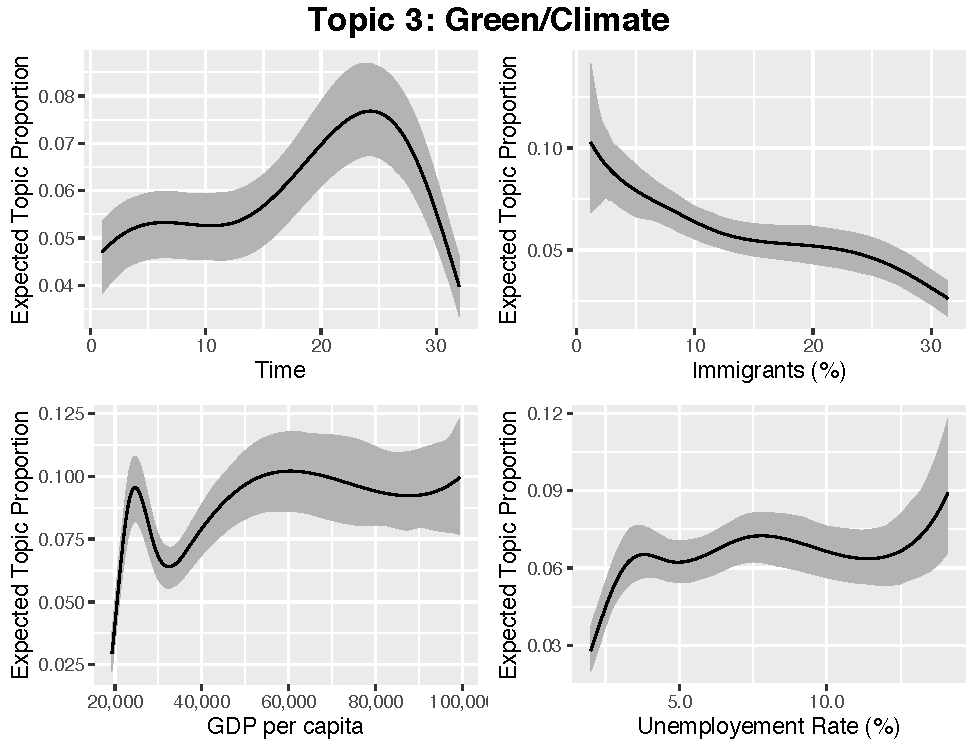
\includegraphics[width=\linewidth]{../plots/appendix/4_4/beta_t3_cont.pdf}
  \end{subfigure}
  \begin{subfigure}[b]{0.4\linewidth}
    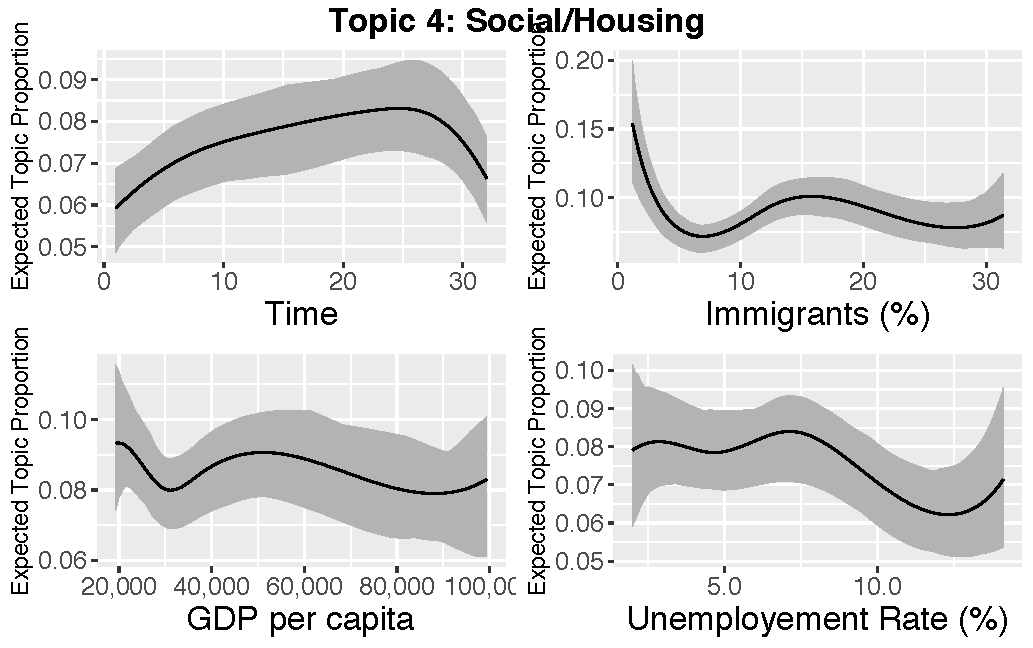
\includegraphics[width=\linewidth]{../plots/appendix/4_4/beta_t4_cont.pdf}
  \end{subfigure}
  \caption{bla}
  \label{fig:coffee}
\end{figure}

\begin{figure}[h!]
  \centering
  \begin{subfigure}[b]{0.4\linewidth}
    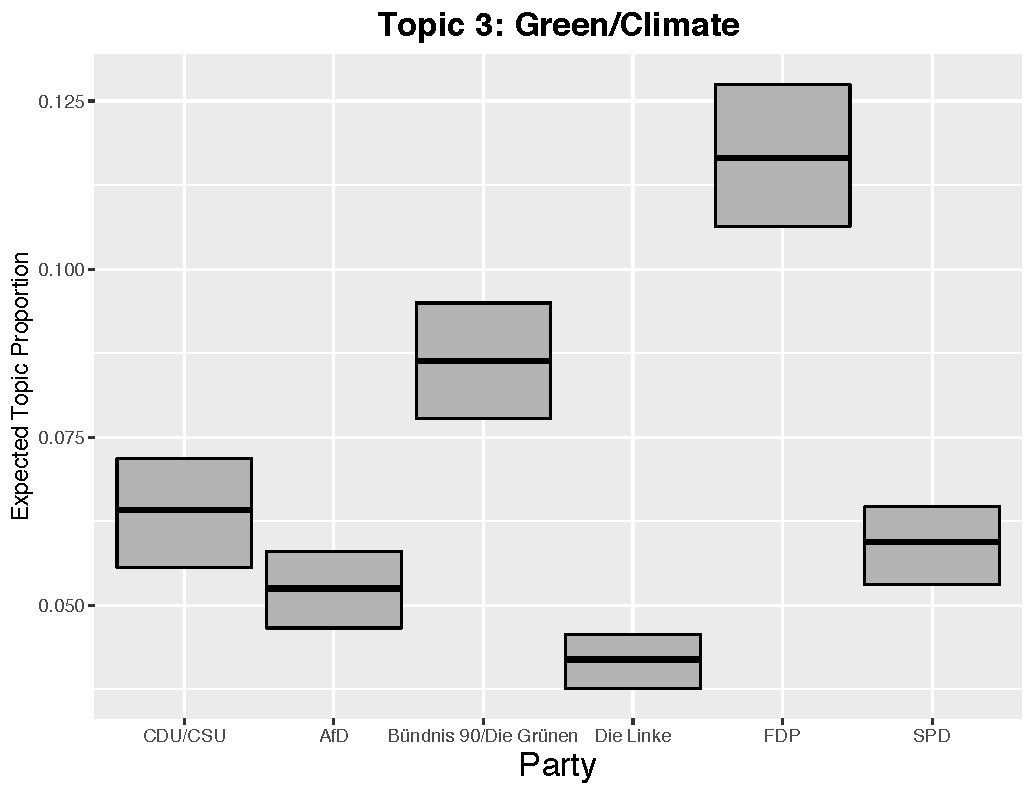
\includegraphics[width=\linewidth]{../plots/appendix/4_4/beta_t3_cat.pdf}
  \end{subfigure}
  \begin{subfigure}[b]{0.4\linewidth}
    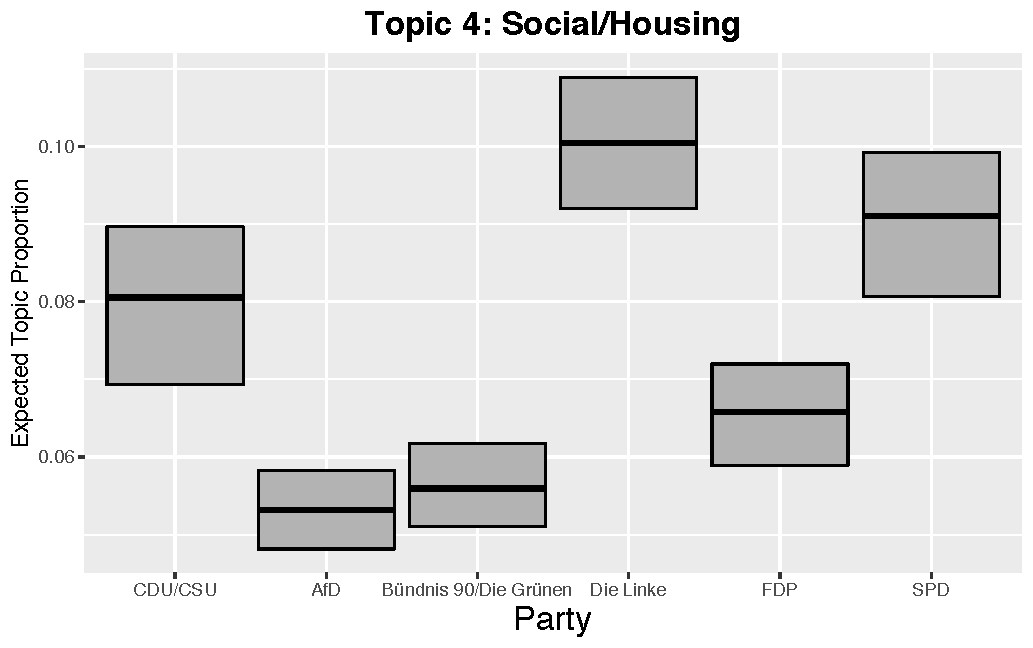
\includegraphics[width=\linewidth]{../plots/appendix/4_4/beta_t4_cat.pdf}
  \end{subfigure}
  \caption{blabla}
  \label{fig:coffee}
\end{figure}

\begin{figure}[h!]
  \centering
  \captionsetup{justification=centering,margin=2cm}
  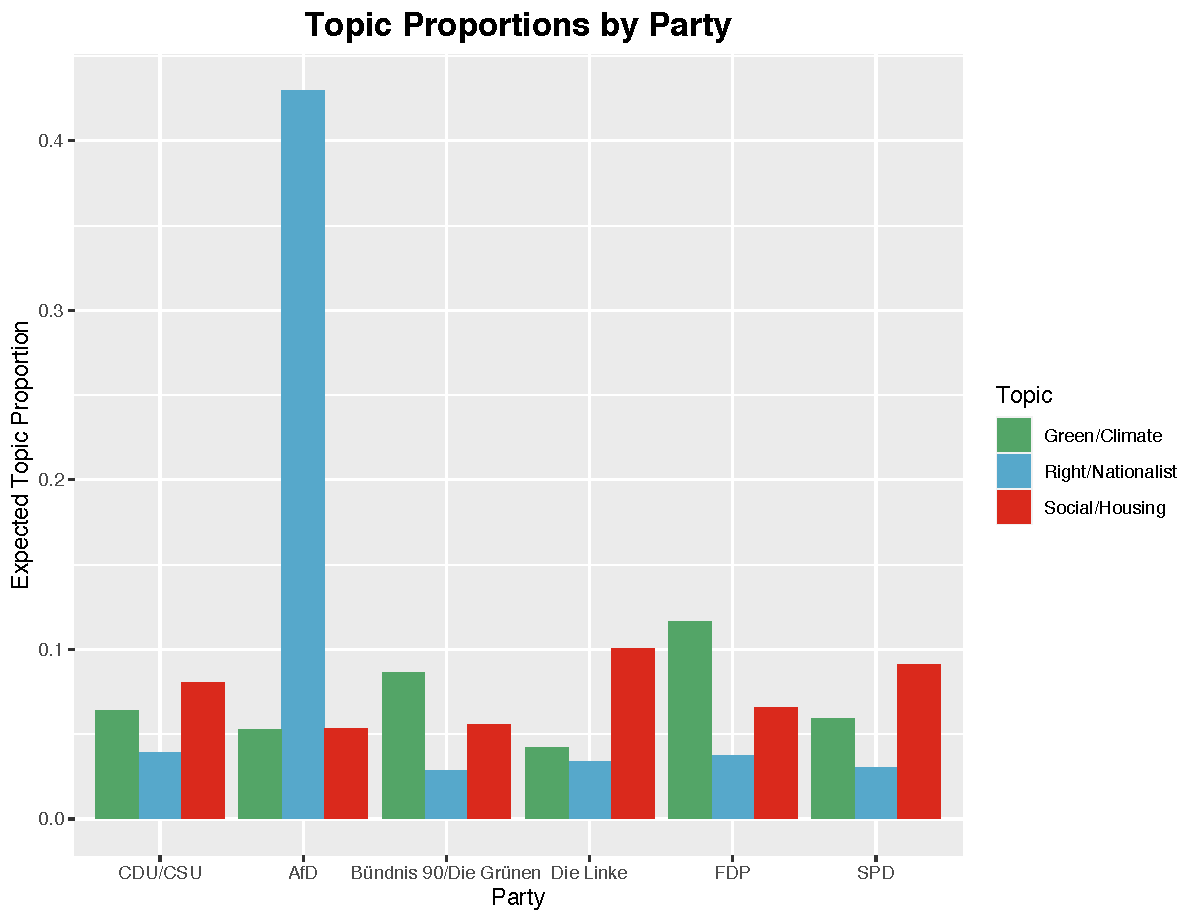
\includegraphics[scale = 0.5]{../plots/appendix/4_4/beta_t134_cat.pdf}
  \caption{Topical prevalence by political party for topics 1, 2, and 3.}
  \label{fig:boat1}
\end{figure}

\begin{figure}[h!]
    \centering
  \begin{subfigure}[b]{0.3\linewidth}
    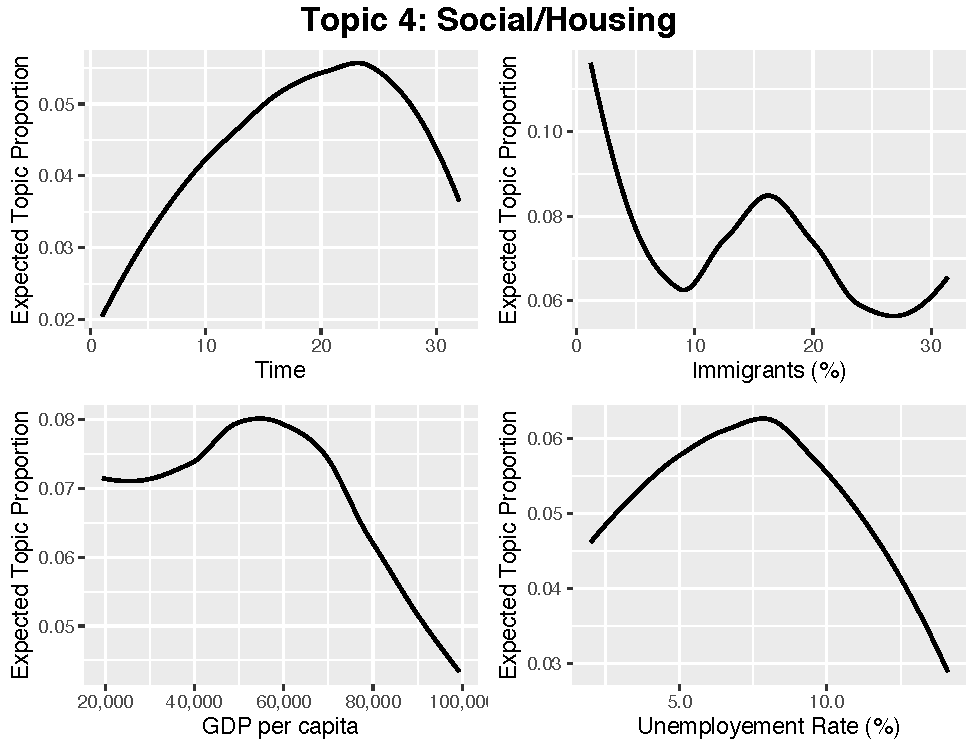
\includegraphics[width=\linewidth]{../plots/appendix/4_4/direct_t4_without_credible.pdf}
  \end{subfigure}
  \begin{subfigure}[b]{0.3\linewidth}
    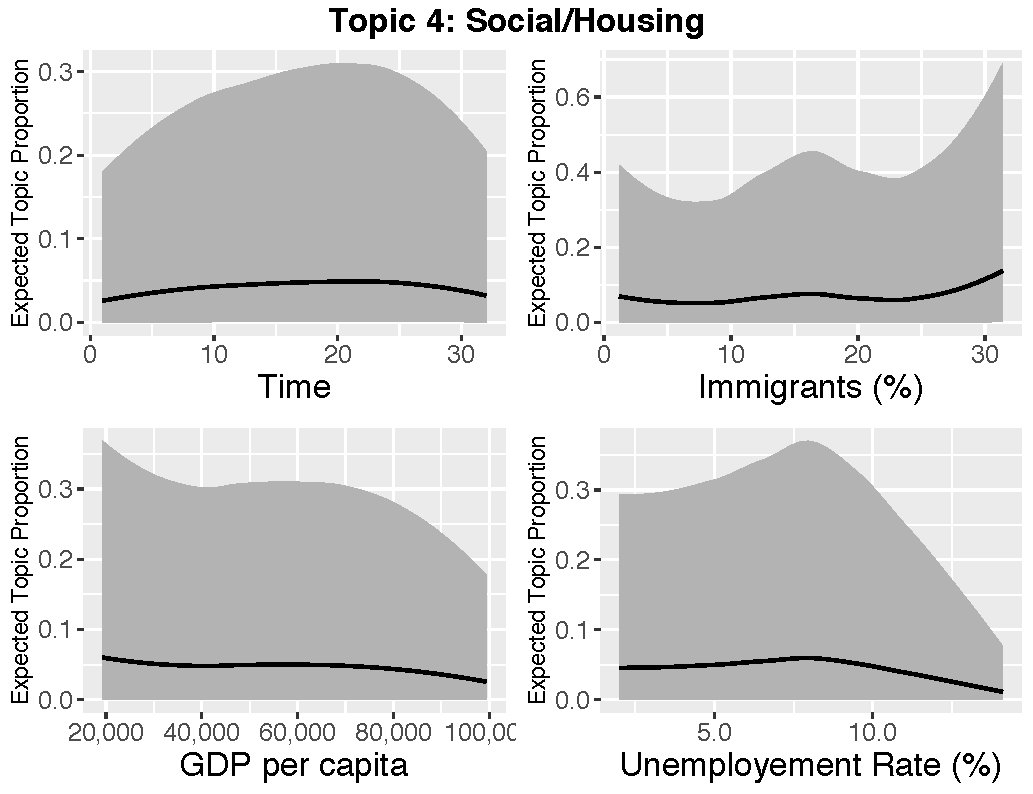
\includegraphics[width=\linewidth]{../plots/appendix/4_4/direct_t4_with_credible.pdf}
  \end{subfigure}
  \begin{subfigure}[b]{0.3\linewidth}
    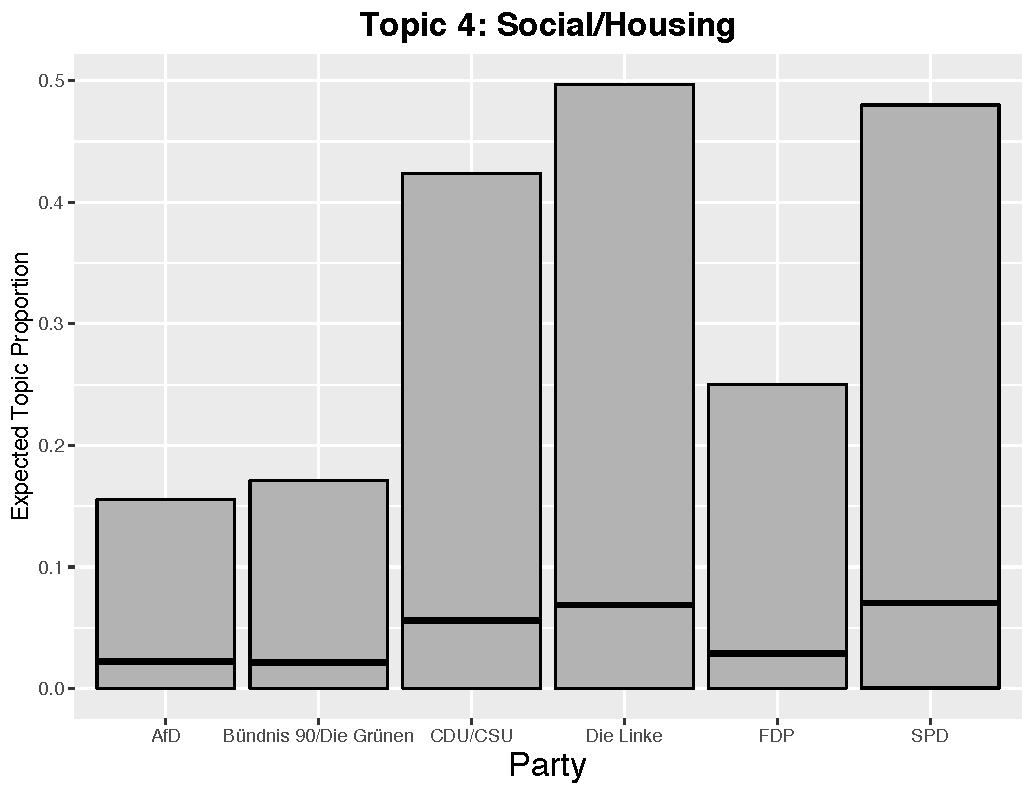
\includegraphics[width=\linewidth]{../plots/appendix/4_4/direct_t4_cat.pdf}
  \end{subfigure}
  \caption{bla}
  \label{fig:coffee}
\end{figure}


\subsubsection*{Additional Figures and Tables of Section 6}

\begin{figure}[h!]
  \centering
  \begin{subfigure}[b]{0.4\linewidth}
    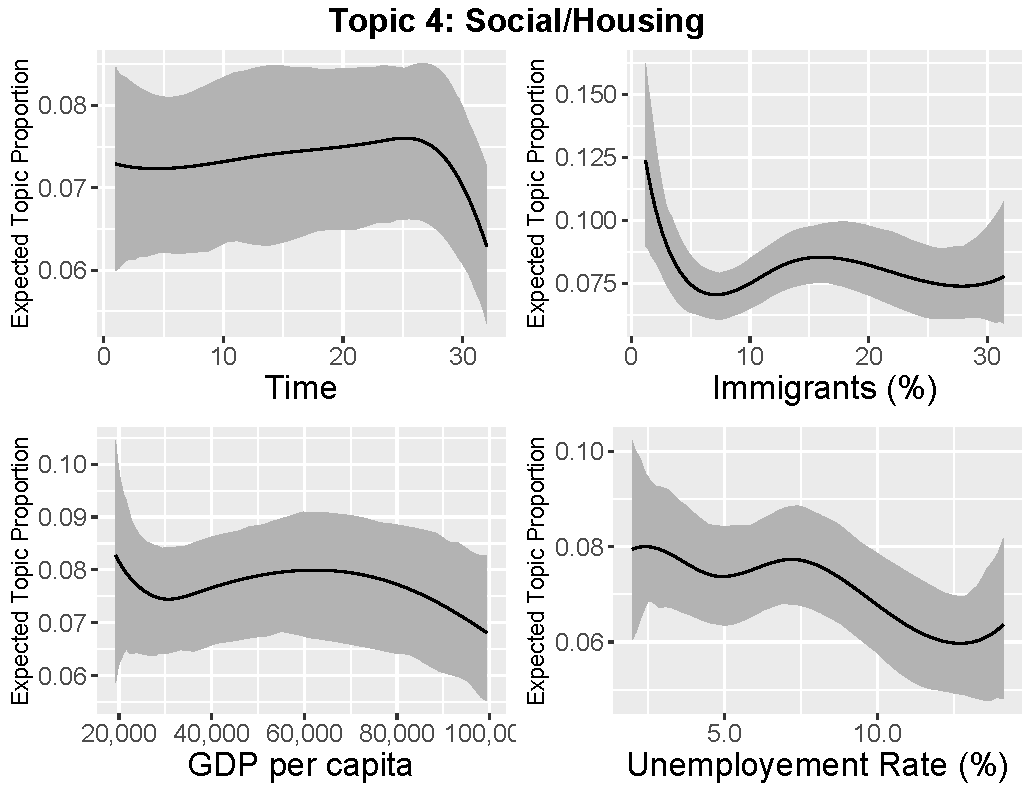
\includegraphics[width=\linewidth]{../plots/appendix/4_6/beta_t4_cont_ctm.pdf}
  \end{subfigure}
  \begin{subfigure}[b]{0.4\linewidth}
    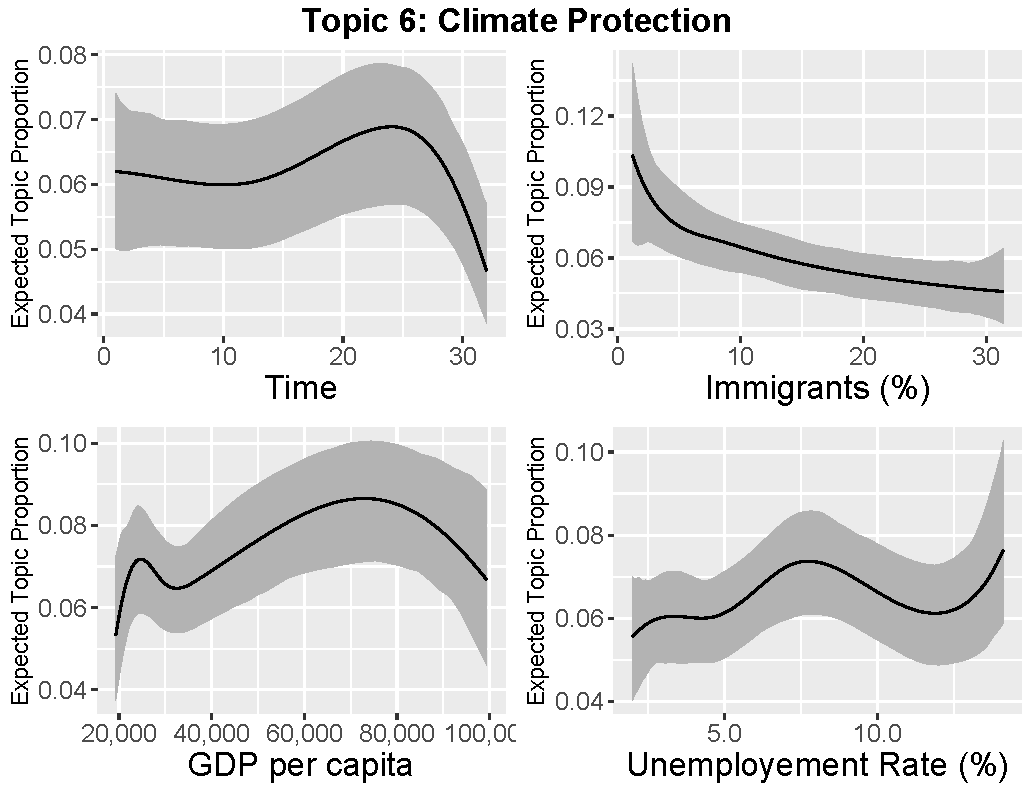
\includegraphics[width=\linewidth]{../plots/appendix/4_6/beta_t6_cont_ctm.pdf}
  \end{subfigure}
  \caption{Mean and 95\% credible intervals for smooth effects, obtained using beta regression (no covariates included in model estimation).}
  \label{fig:beta_t46_cont_ctm}
\end{figure}

\begin{figure}[h!]
  \centering
  \begin{subfigure}[b]{0.4\linewidth}
    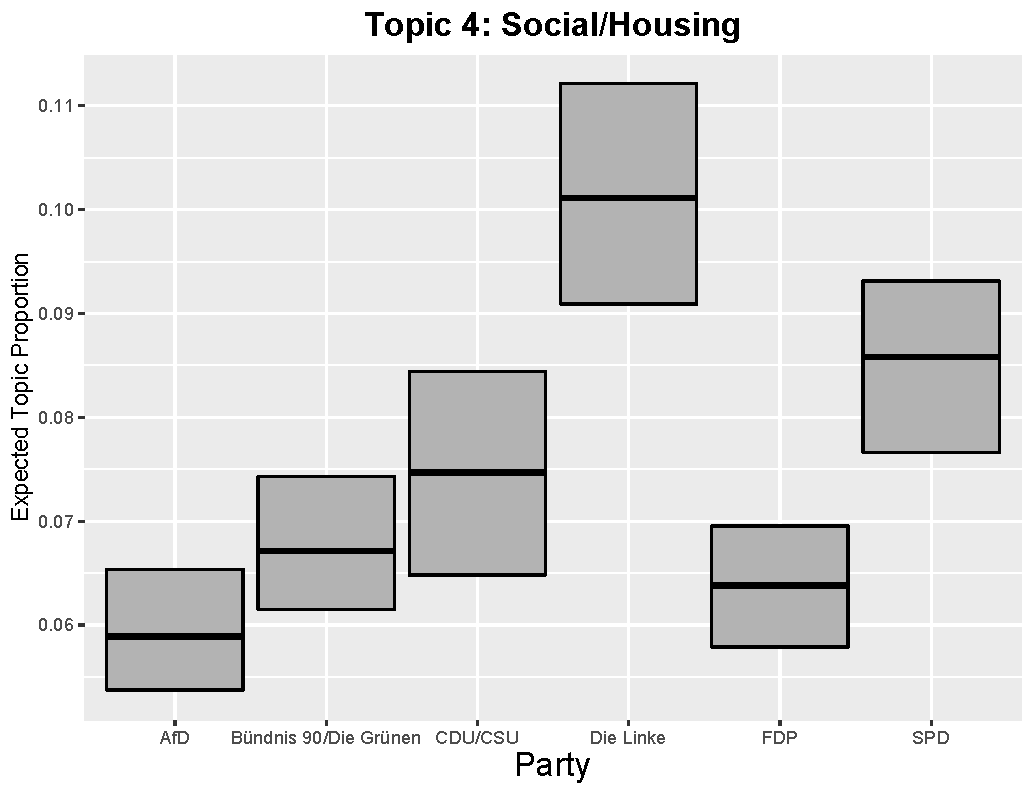
\includegraphics[width=\linewidth]{../plots/appendix/4_6/beta_t4_cat_ctm.pdf}
  \end{subfigure}
  \begin{subfigure}[b]{0.4\linewidth}
    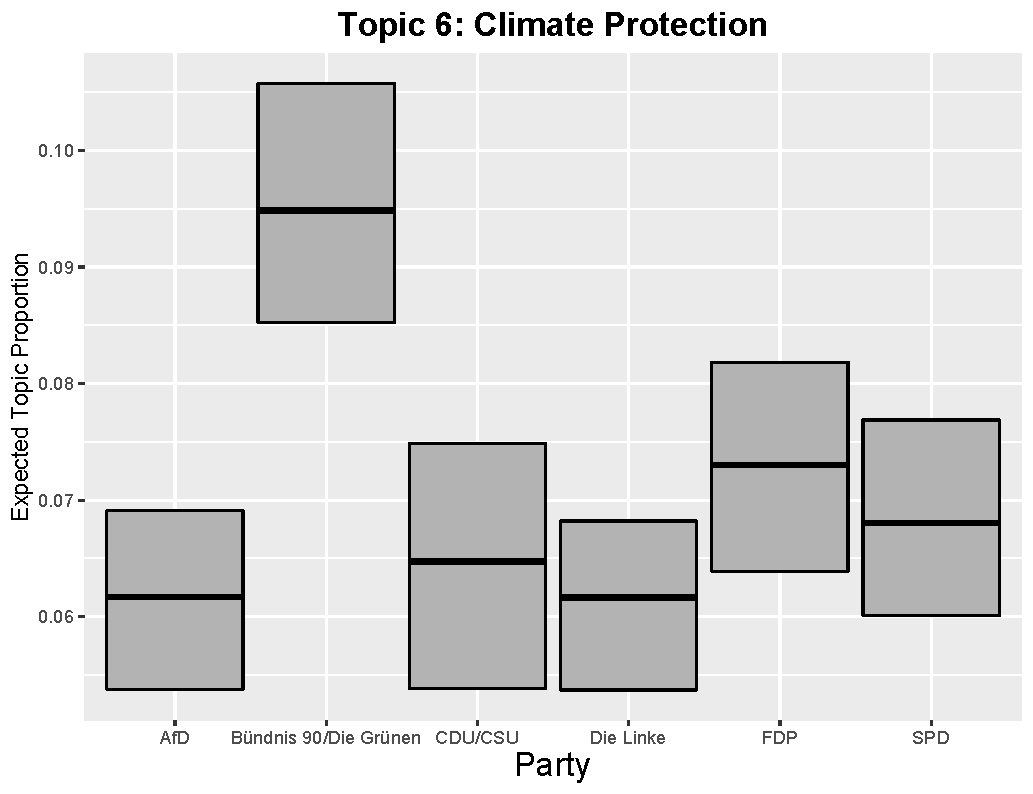
\includegraphics[width=\linewidth]{../plots/appendix/4_6/beta_t6_cat_ctm.pdf}
  \end{subfigure}
  \caption{Mean and 95\% credible intervals for different political parties, obtained using beta regression (no covariates included in model estimation).}
  \label{fig:beta_t46_cat_ctm}
\end{figure}

\begin{figure}[h!]
  \centering
  \captionsetup{justification=centering,margin=2cm}
  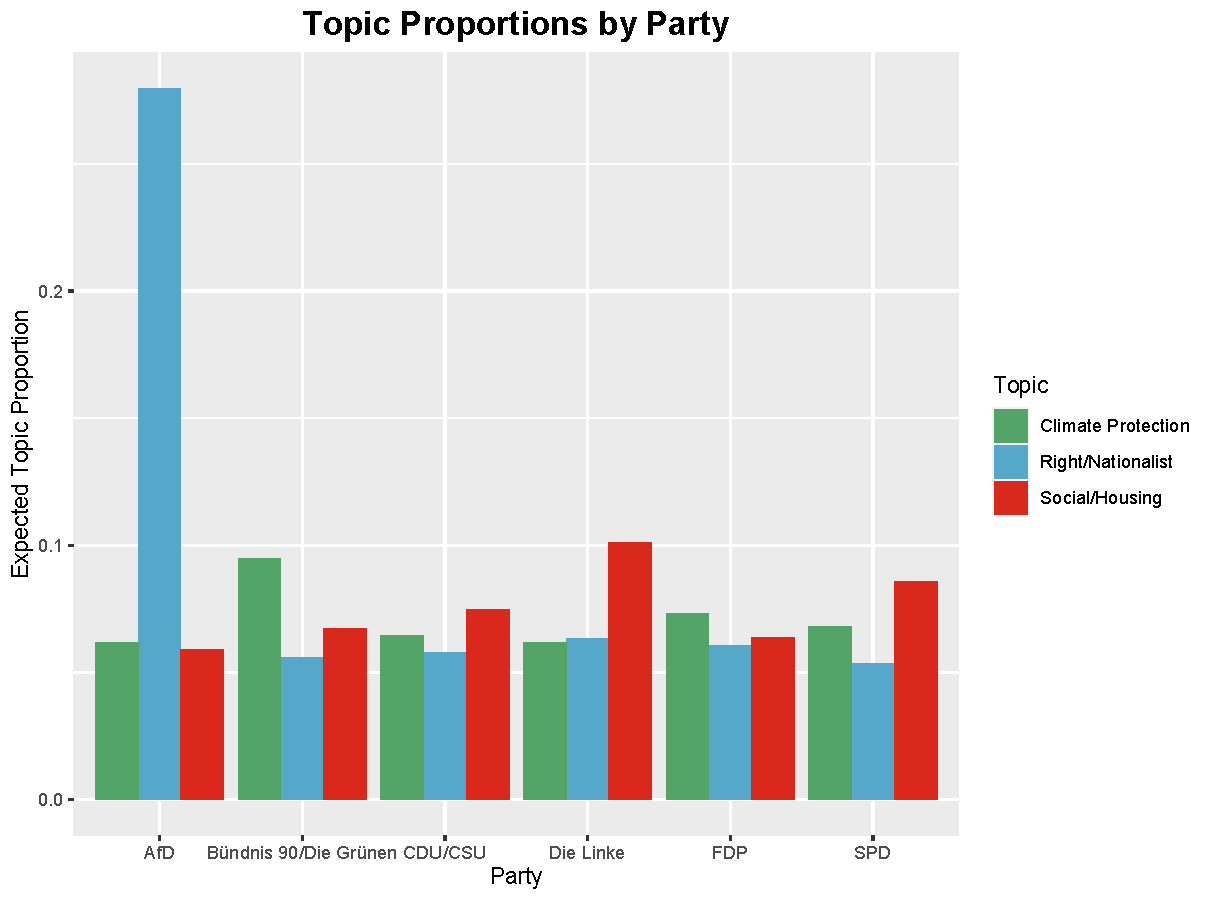
\includegraphics[scale = 0.5]{../plots/appendix/4_6/beta_t146_cat_ctm.pdf}
  \caption{Topical prevalence by political party for topics 1, 4, and 6 (beta regression, no covariates).}
  \label{fig:beta_t146_cat_ctm}
\end{figure}